\chapter{Global Supercoiling in Aevol}
\label{chap:aevol}

\section{Introduction}

\subsection{Motivation}

We want to study the interaction between supercoiling mutations and other  mutations under an epistasis and evolution lens.

- Mutations in the genes regulating supercoiling (henceforth called supercoiling mutations) affect the phenotype globally, as they alter the expression level of many genes at once.

- In experimental evolution settings (E. coli in LTEE), supercoiling mutations have been found to have gone to fixation early in some lineages, and they have been measured to have a positive fitness impact.
This has been interpreted as a blunt adaptation of the gene regulation network of E. coli to its new LTEE-specific environment.

But what happens after those mutations?
Could supercoiling mutations enable subsequent local mutations that wouldn't have been beneficial without these mutations?
That would be a sign of positive epistasis between two kinds of mutations: mutations that affect regulation networks and "baseline" mutations.

In order to detect such an epistasis mechanism, a possible evolutionary signature would be that, along the lineage of an given individual, more genomic mutations happen just after a supercoiling mutation rather than just before.
This would be the sign that the supercoiling mutation is a "jump" through the fitness landscape, allowing for genomic mutations that fine-tune adaptation by locally exploring the new region of the fitness landscape.

\section{Method}

In order to investigate this, we used the digital genetics framework Aevol.
Aevol is a set of tools based upon an individual-based simulation with discrete non-overlapping generations, simulating a population of individuals evolving in a fixed environment.
The Aevol model focuses on precise modeling of the individuals' genome, following the central dogma of molecular biology: individuals have a genome, which is transcribed into RNAs, that are in turn translated into proteins that are assembled into a comprehensive phenotype.
Based on this phenotype, individuals compete for reproduction, and pass their genomes, which undergo random mutations, to the next generation.

\subsection{Changes to the model}

In the classical Aevol model, assuming a constant environment, the phenotype of an individual is fully described by its genetic sequence (in Aevol, a single circular chromosome).

In order to model supercoiling, we started with the simplest mathematical model: each chromosome has a supercoiling level that is constant along the genome and over time, which can be interpreted as the spatial and temporal average of the supercoiling level (which, in real life, varies in both time and space).

To implement this model in Aevol, we changed the genotype of individuals, by adding a single positive real number representing the (average) supercoiling level of this individual's genome.

We represent the supercoiling level of an individual by $\sigma$, and constrain it to be in the interval $[-1, 1]$.
Then, we slightly alter the process for computing the expression level $e$ of a protein.
In vanilla Aevol, this expression level is determined by the distance $d$ of the current RNA's promoter to a baseline promoter, according to the formula: $e = 1 - \frac{d}{1+d_{max}}$, where $d_{max} = 4$, meaning that we allow a maximum of $4$ mutations away from the optimal promoter.

To reflect the biological effect of supercoiling, which is that more tightly wound DNA (more positive $\sigma$) is less transcribed than less tightly wound DNA (more negative $\sigma$), we alter this formula using a linear model:
$e = (1 - \frac{d}{1+d_{max}}) * (1 - \sigma)$.

In this model, $\sigma = 0$ represents the baseline level of supercoiling, resulting in no effect on transcription.

The mutation operator that we chose is a continuous variation model: when an individual reproduces and undergoes the mutation process, we first use a Bernoulli trial with probability $p$ to decide whether its supercoiling level should change or remain constant.
Then, if the individual's supercoiling level is to change, we choose a delta $\delta\sigma$ according to a normal distribution $\mathcal{N}(0, s^2)$, and finally set the supercoiling level $\sigma'$ of the descendant as $\sigma' = \sigma + \delta\sigma$.
The parameters of these laws are given as parameters to the Aevol simulation, with typical values $p = 10^{-1}$ and $s^2 = 10^{-2}$.

\subsection{Experimental protocol}

In order to measure the possible difference in the number of genomic mutations happening in a lineage just before and after a supercoiling mutation, we adopted the following experimental protocol.

We ran 5 replicas of the evolution of a population of 1,024 individuals, initialized as clones of a random genome that has at least one good gene, and an initial value of supercoiling of zero, for 1,000,000 generations.

At the end of the experiment, we retrace the evolutionary lineage of a focal individual in the population, and list all the mutations that have happened since its original ancestor.

(Note: it is fine to choose any individual rather than the best of the last generation, as a population of 1,024 haploid individuals should coalesce in around 1,000 generations.)

Then, for each of the mutation operators in Aevol, we measured the time since the previous and before the next mutation (of any type).

\pagebreak

\section{Results}

\subsection{Evolution of the populations}

\begin{figure}[h!]
  \centering
  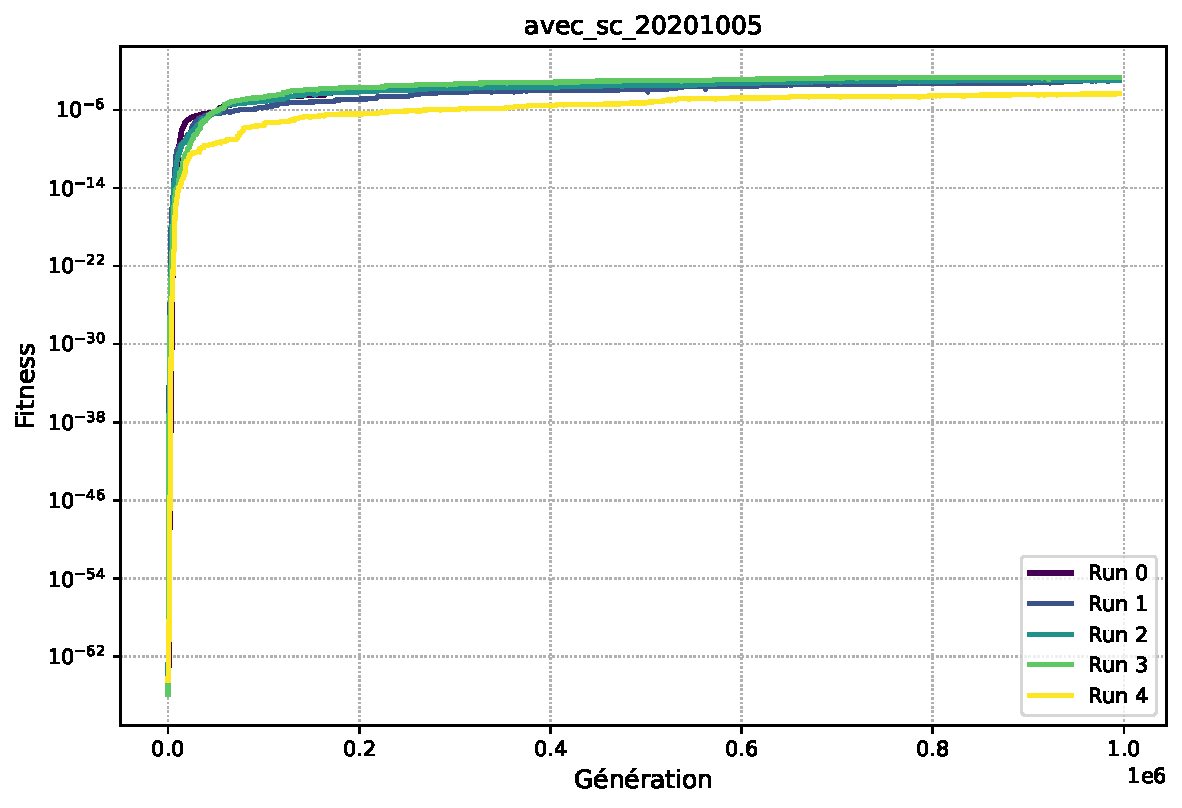
\includegraphics[width=0.75\textwidth]{aevol/images/fitness_agrege.pdf}
  \caption{Fitness of the lineage of the focal individual.}
  \label{fig:fitness}
\end{figure}

Figure~\ref{fig:fitness} shows the fitness of the lineage of the focal individual over the 1M generations of each run.
Two evolutionary phases are distinguishable: during the first 100,000 to 200,000 generations, fitness increases very quickly.
Then, over the last 800,000 generations, fitness increases much more slowly, but never completely stops doing so.


\subsection{Evolution of the supercoiling level}

\begin{figure}[h!]
  \centering
  \begin{subfigure}[b]{0.49\textwidth}
    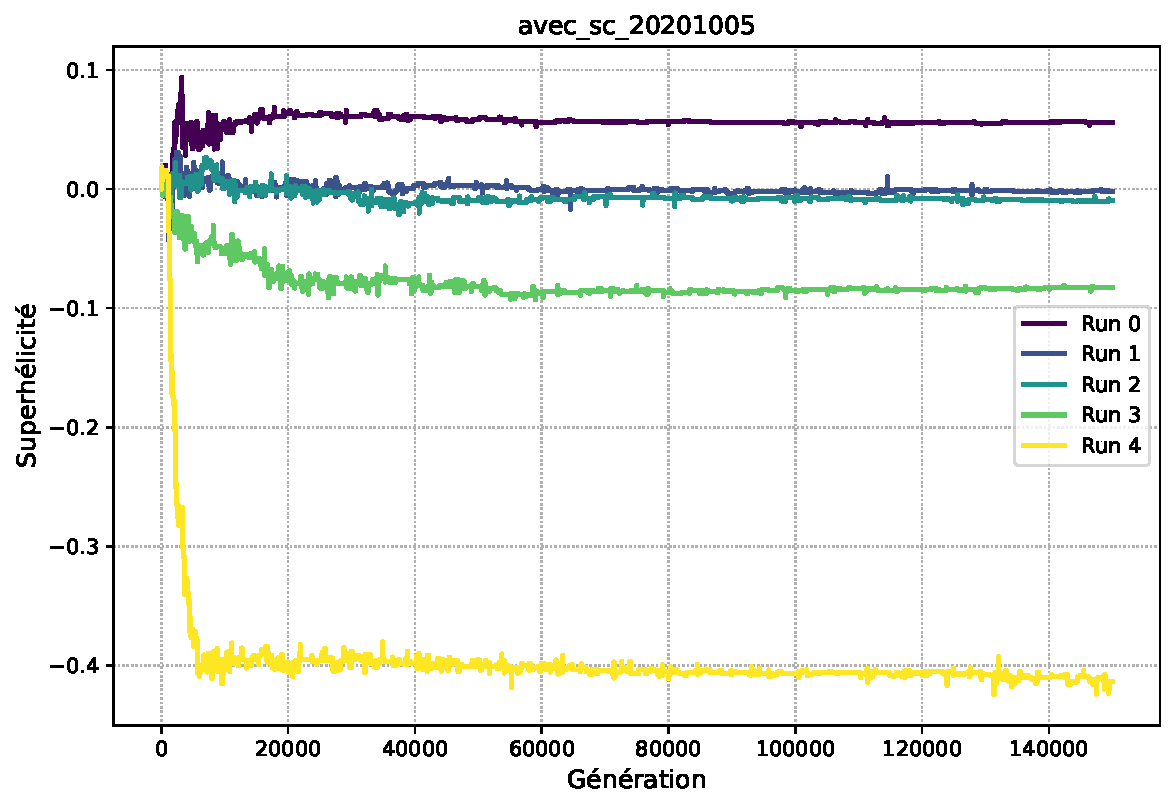
\includegraphics[width=\textwidth]{aevol/images/superhelicite_agrege_zoom.pdf}
    \caption{Zoom on the first 150,000 generations.}
    \label{fig:sc_zoom}
  \end{subfigure}
  \begin{subfigure}[b]{0.49\textwidth}
    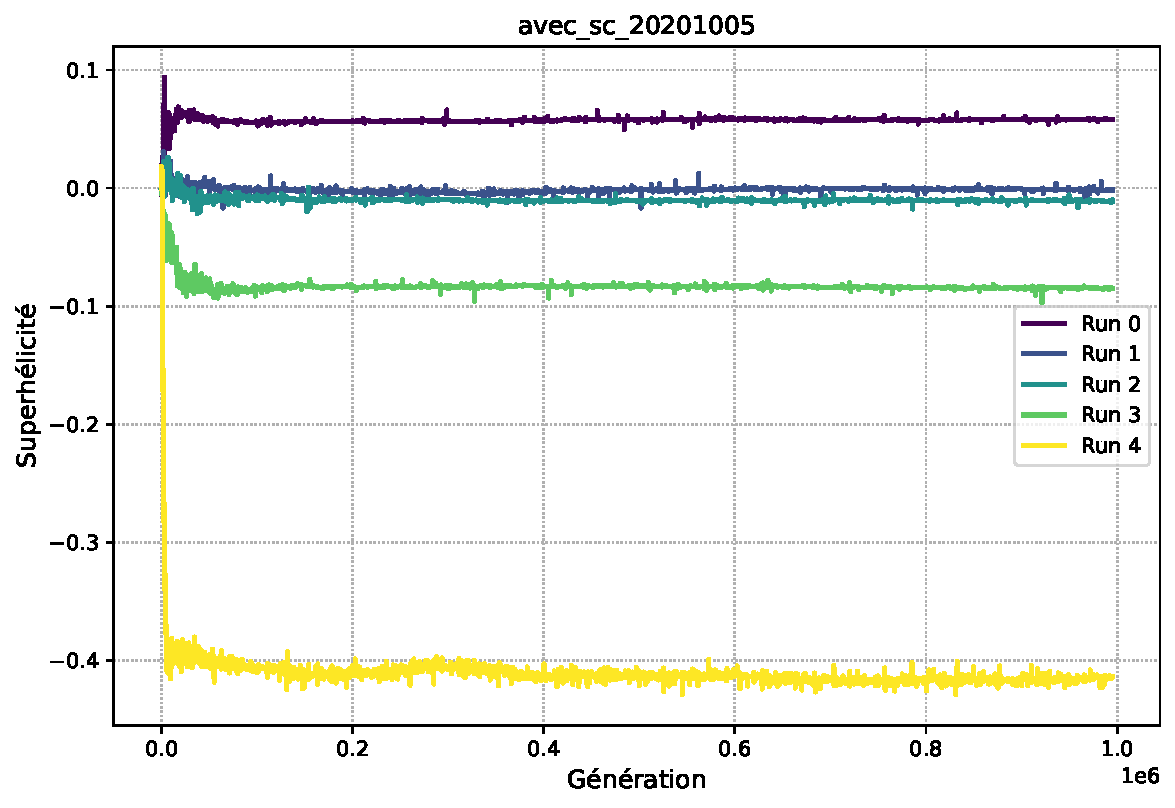
\includegraphics[width=\textwidth]{aevol/images/superhelicite_agrege.pdf}
    \caption{Evolution over the complete runs.}
    \label{fig:sc_all}
  \end{subfigure}
  \caption{Evolution of the supercoiling level in the lineage of the focal individual of each run.}
  \label{fig:sc}
\end{figure}

Figure~\ref{fig:sc} shows the evolution of the supercoiling level of the lineage of the focal individual during each of the 5 runs.
With the global supercoiling model, we observe that supercoiling stabilizes very quickly, in the 100,000 first generations of evolution, and remains nearly constant afterwards.

We interpret this as a coevolutionary process between the genome and the global supercoiling level, until the genome evolution starts to slow down.
Indeed, when the phenotype is already well-matched to the environment, a variation of the supercoiling level in this model alters the phenotype (the size of the triangles) at all points of the phenotypic space, tweaking supercoiling mutations towards being much more harmful than beneficial.

This quick stabilization of the supercoiling level seems to be a first sign that the global supercoiling model is too simplistic to express interesting evolutionary behaviors for the supercoiling system.

\subsection{Average times before and after mutations}

In this section, we look at the distribution of the time since the previous mutation and before the next mutation, for each kind of mutation, in the lineage of the focal individual: if these are significantly different, this might signal that a kind of mutation accelerates (or slows) down evolution.

Moreover, since we are observing the lineage of an individual, not all fixed mutations are beneficial: most of them are neutral, and some are harmful.

\begin{figure}[h!]
  \begin{subfigure}[t]{0.49\textwidth}
    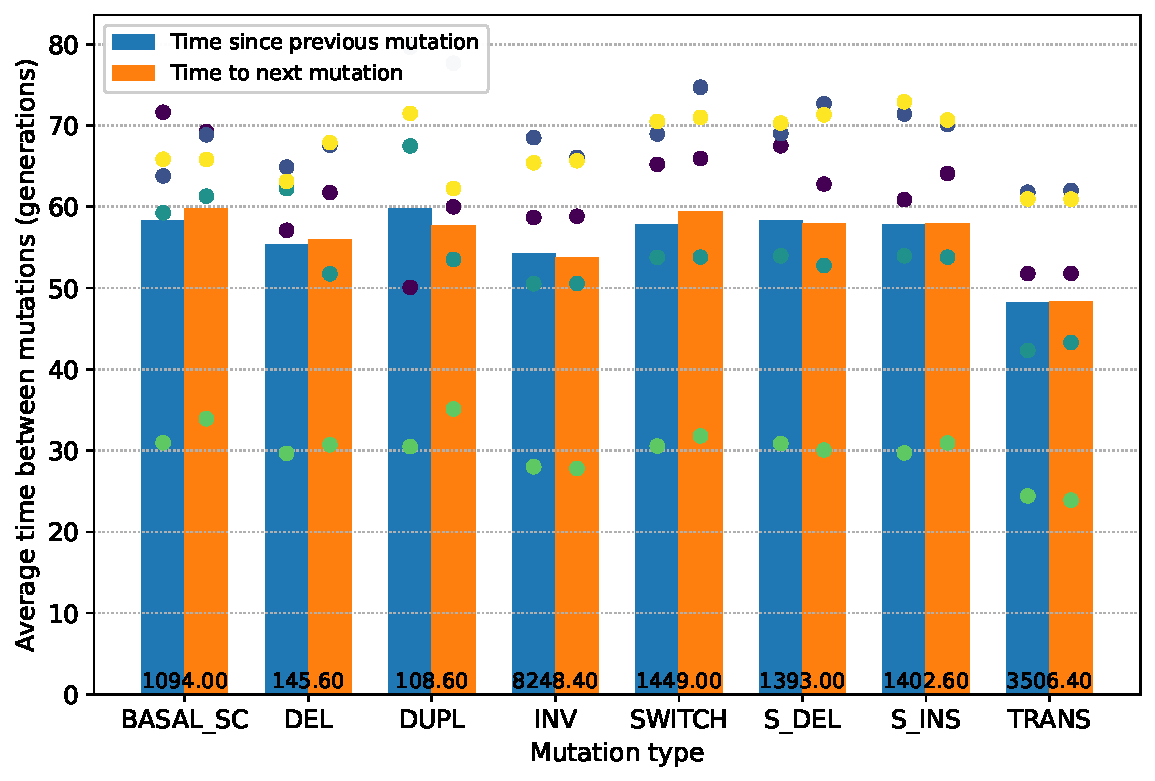
\includegraphics[width=\textwidth]{aevol/images/with_sc_mut_time_150k_995k.pdf}
    \caption{With supercoiling, with neutral mutations}
    \label{subfig:sc_neut}
  \end{subfigure}
  \begin{subfigure}[t]{0.5\textwidth}
    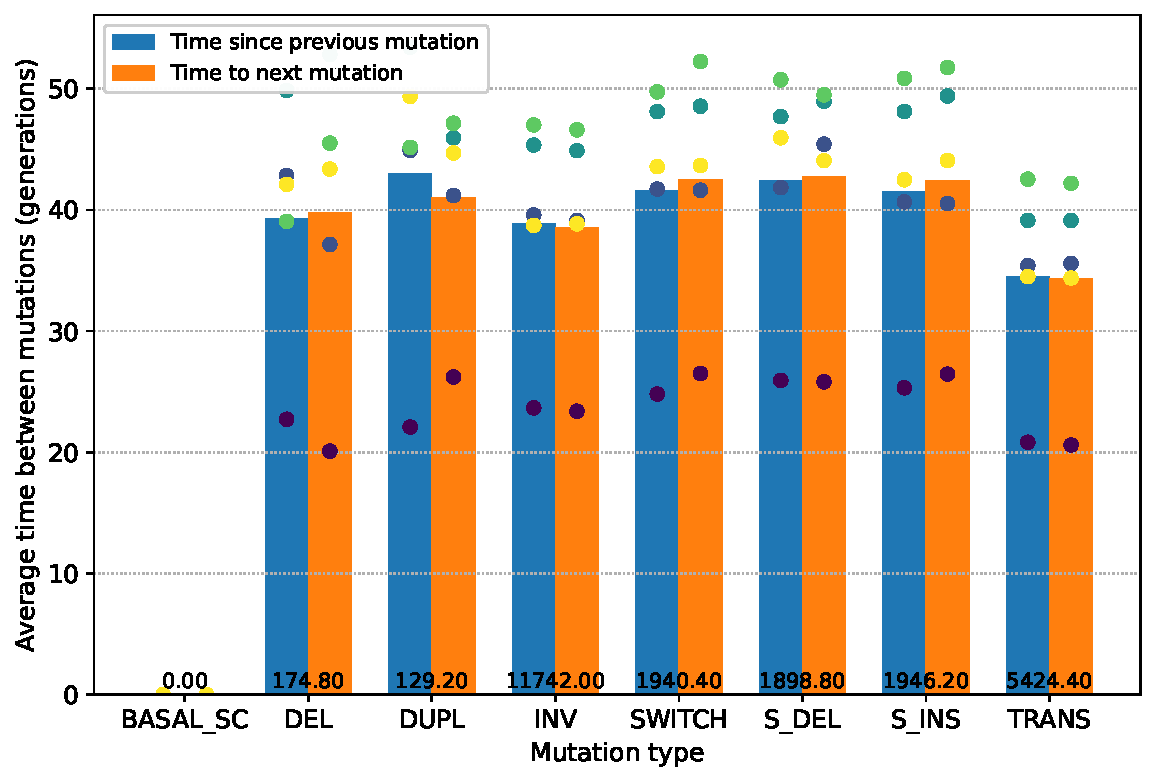
\includegraphics[width=\textwidth]{aevol/images/without_sc_mut_time_150k_995k.pdf}
    \caption{Without supercoiling, with neutral mutations}
    \label{subfig:no_sc_neut}
  \end{subfigure}

  \begin{subfigure}[b]{0.49\textwidth}
    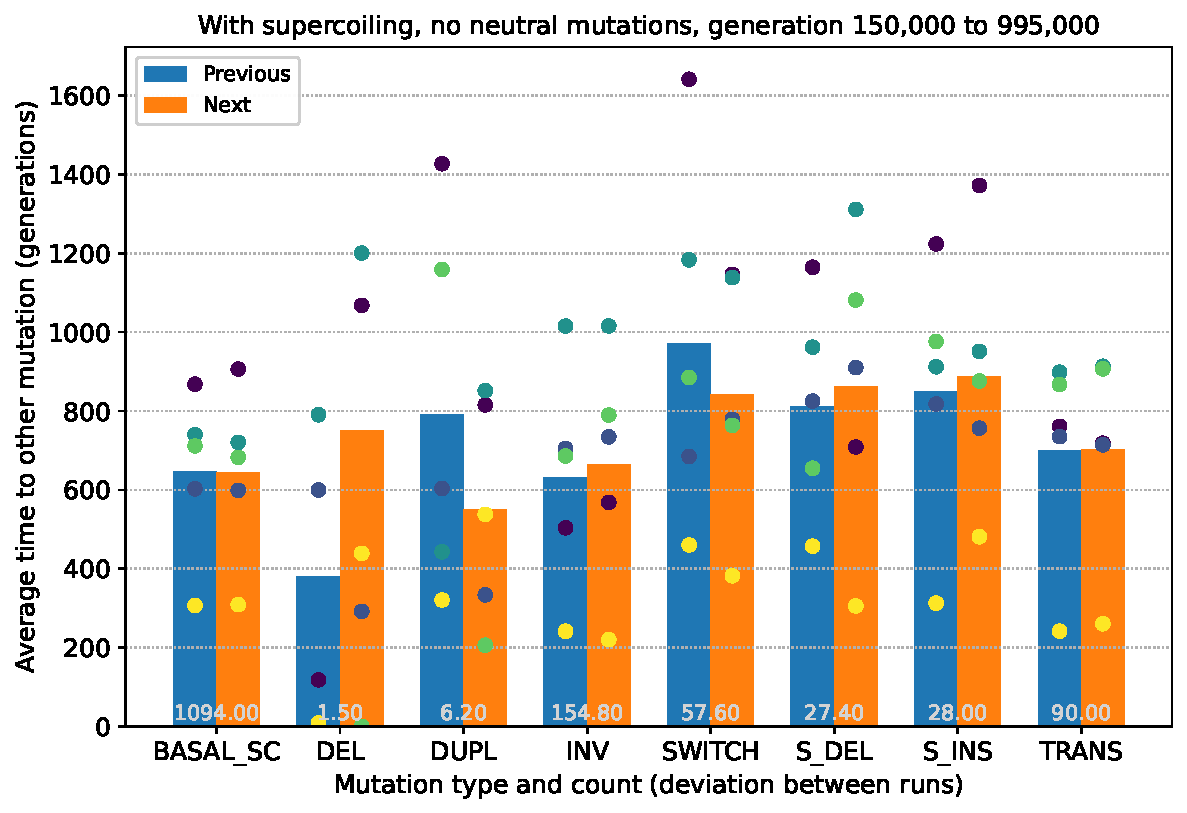
\includegraphics[width=\textwidth]{aevol/images/with_sc_mut_time_no_neutral_150k_995k.pdf}
    \caption{With supercoiling, without neutral mutations}
    \label{subfig:sc_no_neut}
  \end{subfigure}
  \begin{subfigure}[b]{0.49\textwidth}
    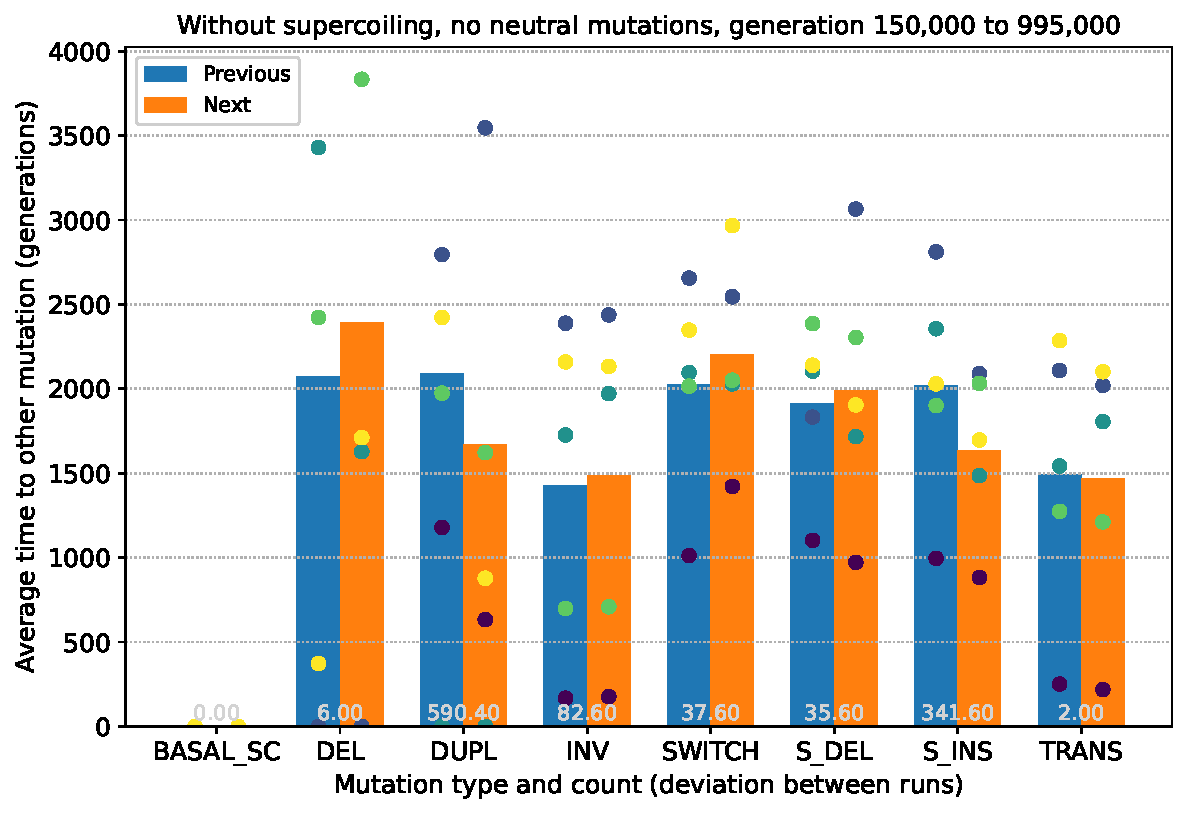
\includegraphics[width=\textwidth]{aevol/images/without_sc_mut_time_no_neutral_150k_995k.pdf}
    \caption{Without supercoiling, without neutral mutations}
    \label{subfig:no_sc_no_neut}
  \end{subfigure}

  \caption{Average times before and after each type of mutation, in the experimental (left column) and control (right column) groups, including (top row) or excluding (bottom row) neutral mutations. Each color represents one of the 5 runs.}
  \label{fig:mut_times}
\end{figure}

Figure~\ref{fig:mut_times} summarizes these results.
As we can see in figures~\ref{subfig:sc_neut} and~\ref{subfig:sc_no_neut}, it does not look like mutation times after a supercoiling mutation are significantly lower than before supercoiling mutations, suggesting that under this model supercoiling mutations do not play a potentiating role.

This seems true whether looking at the mutation times including all mutations, or including only non-neutral mutations, which are under selection.

In figures~\ref{subfig:sc_neut} (resp.~\ref{subfig:no_sc_neut}), the pale green (resp. deep purple) run shows significantly lower mutation times than the other ones.
This can be explained by the fact that the genome of individuals in this lineage are larger than in the other runs, mechanically increasing the number of mutations (the mutation rate per generation is proportional to the genome size), and therefore reducing the delay between mutations.

On the contrary, we can distinguish an effect in large-scale duplications and deletions (most clearly when looking only at non-neutral mutations): mutations happen faster after a duplication than before (smaller time to the next mutation), but slower after a deletion (larger time to next mutation).
This might however due to the effect of these mutations on genome size, as larger genomes statistically undergo more mutations.

\section{Discussion}

This preliminary work, modeling supercoiling as constant in time and space, is not sufficient to show that mutations in the supercoiling regulation system can impact the evolutionary trajectory of a population.

Indeed, many aspects of the biology of supercoiling are left out in this model, most notably the transcription-supercoiling coupling: gene transcription locally affects the supercoiling level in a chromosome, resulting in complex coupling between the transcription level of neighboring genes.

The next step would therefore be to create a model of supercoiling comprising local variations in the supercoiling level, to allow for supercoiling mutations to have non-linear phenotypic effects; then, to incorporate this model into Aevol and determine to which level selection acts upon these mutations.
